% ============================================================
% Reporte: datapath-1
% Generado a partir de reportes/comun/plantilla_base.tex
% (NO edites la plantilla: cada unidad trabaja en su main.tex)
%
% Reglas de secciones y extensiones: reportes/AGENTS.md
% Compilar SIEMPRE con:
%   ../../scripts/latexbuild main.tex      (desde esta carpeta)
%   → genera build/main.pdf
% ============================================================
\documentclass[llncs]{llncs}

\usepackage[utf8]{inputenc}
\usepackage[T1]{fontenc}
\usepackage{fontspec}
\setmonofont{DejaVu Sans Mono}
\usepackage{graphicx}
\usepackage{amsmath}
\usepackage{tikz}
\usetikzlibrary{arrows.meta,positioning}
\usepackage{listings}
\usepackage{xcolor}
\usepackage{hyperref}
\hypersetup{
  hidelinks,
  colorlinks=false,
  pdfborder={0 0 0},
  bookmarksnumbered=true
}

% ---- Encabezado del resumen en español (llncs lo pone en inglés) ----
\renewcommand{\abstractname}{Resumen.}
\renewcommand{\andname}{,}
\renewcommand{\lastandname}{\unskip,}
\renewcommand{\refname}{Referencias}
\renewcommand{\tablename}{Tabla}
\renewcommand{\lstlistingname}{Listado}

% ---- Estilo para código VHDL (apéndice y fragmentos) ----
\lstdefinestyle{vhdl}{
  language=VHDL,
  basicstyle=\ttfamily\fontsize{9}{10.5}\selectfont,
  keywordstyle=\color{black},
  commentstyle=\color{black}\itshape,
  stringstyle=\color{black},
  showstringspaces=false,
  breaklines=false,
  breakatwhitespace=false,
  columns=fullflexible,
  keepspaces=true,
  frame=single,
  rulecolor=\color{black},
  xleftmargin=0.6em,
  xrightmargin=0.6em
}
\lstset{style=vhdl}
\setlength{\emergencystretch}{2em}

\begin{document}

% ============================================================
% TÍTULO Y AUTORES
% ============================================================
\title{Diseño y Verificación en {VHDL} de un Datapath de 8~Bits:
Datapath 1 --- MUX, ALU, Registro Realimentado y Buffer de Salida}

\author{Aldo Mauricio Villegas Peralta\and
Uriel Lemus Pérez\and
Max Ramos Martínez\and
Alfredo Ramírez Candia\and
Santiago Silverio Flores}

\authorrunning{Villegas Peralta et al.}
\institute{Equipo de Arquitectura de Computadoras,\\
Benemérita Universidad Autónoma de Puebla, Puebla, México\\
\email{\{vp202368617, lp202362797, rm202376182, rc202375947, sf202367190\}@alm.buap.mx}}

\maketitle

% ============================================================
% RESUMEN  (< 100 palabras — fuente 9pt con sangría, estilo llncs)
% ============================================================
\begin{abstract}
Se diseña y verifica por simulación un datapath de 8~bits con MUX
de entrada, ALU de tres operaciones ($n+x$, $2n+x$, $n+1$), registro con
carga realimentado a la ALU y buffer tri-estado de salida. El circuito se
describe en VHDL-2008 y se valida con cinco bancos de prueba autochequeados
en GHDL, analizando las ondas con GTKWave. Bajo el modelo especificado, las
operaciones, la carga, la retención con $L=0$ y la alta impedancia se
comportan como se esperaba; la aritmética es módulo $2^8$ sin banderas.
\end{abstract}

\noindent\textbf{Palabras Clave:} Arquitectura de Computadoras, Datapath,
VHDL, Simulación, GHDL

% ============================================================
% 1. INTRODUCCIÓN  (1–2 cuartillas)
% ============================================================
\section{Introducción}
\label{sec:intro}

Para afrontar el diseño de sistemas digitales, la ingeniería recurre a
abstracciones por capas: quien escribe código ve instrucciones y no
transistores, y quien diseña la unidad de procesamiento la compone a partir
de bloques funcionales delimitados~\cite{patterson2017cod}. En esa
descomposición, la unidad central de procesamiento (CPU) se separa
convencionalmente en una ruta de datos o \emph{datapath}, encargada de
transportar y transformar los datos, y una unidad de control, que secuencia
las operaciones~\cite{hamacher2002co}. Las implementaciones de referencia de
ciclo único ilustran exactamente esta separación: un datapath formado por
MUX, ALU y registros, gobernado por una unidad de control que genera una
palabra de control por ciclo~\cite{patterson2017cod,bryant2015csapp}.
El crecimiento sostenido del número de transistores~\cite{hennessy2017qa} ha
desplazado buena parte del esfuerzo de diseño hacia la descripción y la
verificación automatizadas: antes de construir, el circuito se modela en un
lenguaje de descripción de hardware y se valida por simulación. En el marco
del curso de Arquitectura de Computadoras, este trabajo toma el circuito de
datapath propuesto en el material de clases ---cuyo esquema muestra un MUX
de entrada, una ALU con tres operaciones, un registro con carga y un buffer
de salida con habilitación--- y lo desarrolla como un modelo VHDL-2008
completo~\cite{ieee1076_2008} verificado con bancos de prueba
autochequeados en GHDL~\cite{ghdl-docs} y analizado con
GTKWave~\cite{gtkwave-docs}.

El datapath resultante es una ruta de datos de 8 bits, parametrizable por
medio de un genérico, con cuatro bloques: un MUX $2\to1$ que elige entre un
valor externo y la constante cero; una ALU que implementa tres operaciones
sobre sus dos operandos ($n+x$, $2n+x$ y $n+1$); un registro síncrono con
carga y reinicio; y un buffer tri-estado que conecta la salida externa. La
secuencia no la genera ninguna máquina de estados: una palabra de control de
seis bits distribuidos en cuatro campos, aplicada directamente por el
entorno de simulación, distribuye
el bit de habilitación de salida, la carga del registro, la selección del
MUX y el código de operación de la ALU. Ese alcance es deliberado: sin
unidad de control ni autómata finito~\cite{mano2016lcdf}, se modela y verifica
únicamente la ruta de datos, que es el componente ejecutor del
computador~\cite{hamacher2002co}.

Los objetivos del trabajo son: (i)~describir en VHDL-2008 los módulos del
datapath (MUX, ALU, registro y buffer) con ancho parametrizable;
(ii)~integrarlos en una entidad estructural con la realimentación del
registro hacia la ALU y el desempaquetado de la palabra de control;
(iii)~verificar cada módulo y el conjunto con bancos de prueba
autochequeados; (iv)~analizar el comportamiento temporal observado en las
ondas de simulación; y (v)~documentar el formato de la palabra de control,
las operaciones de la ALU y los límites aritméticos del diseño.

El artículo se organiza como sigue. La Sección~\ref{sec:diseno} presenta el
marco teórico, la arquitectura y los módulos VHDL. La
Sección~\ref{sec:propuesta} describe la propuesta experimental y las
herramientas. La Sección~\ref{sec:simulaciones} muestra las simulaciones, la
Sección~\ref{sec:resultados} analiza los resultados y la
Sección~\ref{sec:conclusiones} recoge las conclusiones y el trabajo
futuro.

% ============================================================
% 2. DISEÑO TEÓRICO  (3–5 cuartillas)
% ============================================================
\section{Diseño Teórico}
\label{sec:diseno}

\subsection{Marco teórico}

El datapath es el bloque de la CPU que ejecuta las operaciones sobre los
datos: mueve operandos, los transforma y almacena resultados. Por sí solo no
decide qué hacer: recibe de la unidad de control una serie de señales que
configuran sus MUX, su ALU y sus registros ciclo a
ciclo~\cite{hamacher2002co,patterson2017cod}. En los diseños de libro esa
unidad de control se modela habitualmente como una máquina de estados de
estilo Moore o Mealy~\cite{mano2016lcdf,harris2015ddca,brown2009fdld,roth2013fld};
formalmente, un autómata finito es una quíntupla de estados, entradas,
función de transición, estado inicial y estados finales~\cite{roth2013fld}, y
las señales de control se reparten en campos codificados dentro de una
microinstrucción~\cite{katz2005cld,wakerly2005ddpp}.

Este trabajo prescinde de esa unidad de control, por criterio del alcance
del encargo: se modela únicamente la ruta de datos y la palabra de control
se aplica desde el banco de pruebas. La consecuencia metodológica es que
cada micro-operación se define como una palabra concreta del puerto
\texttt{cw}, lo que hace el comportamiento del circuito completamente
determinista y directamente verificable sin necesidad de programar un
secuenciador.

En el lado secuencial, el único elemento de memoria es un registro con
habilitación de carga que trabaja de forma síncrona~\cite{mano2016lcdf}; su
modelado recurre a los procesos y a las sentencias condicionales y de caso
del lenguaje~\cite{ashenden2008vhdl}. La salida del conjunto se habilita
mediante un buffer tri-estado, que deja el bus en alta impedancia
(`\texttt{Z}') cuando no está activo~\cite{wakerly2005ddpp};
los nueve valores de la lógica resoluble que incluyen esa alta impedancia
están definidos por el paquete \texttt{std\_logic\_1164} del
estándar~\cite{ieee1164_1993}.

Por su parte, la ALU combina operaciones aritméticas y de corrimiento
dentro de un mismo bloque~\cite{rabaey2002dic}. Existen estructuras
dedicadas, los \emph{barrel shifters}, que desplazan $N$ posiciones en un
solo ciclo~\cite{katz2005cld}, pero el circuito de origen no incluye un
shifter independiente: la única operación de corrimiento necesaria ---el
desplazamiento de un bit que produce el doble de $n$--- se implementa
dentro de la propia ALU (§\ref{sec:alu-op}).

\subsection{Arquitectura general}
\label{sec:arquitectura}

La Fig.~\ref{fig:arquitectura} muestra la arquitectura propuesta. El valor
externo \texttt{dato\_ext} y la constante cero compiten en un MUX $2\to1$
controlado por el campo \texttt{M}; su salida es el operando $A$ de la ALU.
El operando $B$ proviene de la realimentación: es la salida $Q$ del
registro, que por eso almacena el valor $n$. La ALU, gobernada por el campo
\texttt{C}, produce el resultado combinacional $F_{ALU}$, que entra como
dato $D$ del registro. Este se actualiza en el flanco de subida de
\texttt{clk} cuando la habilitación \texttt{L} lo permite, y su salida
$Q$---además de realimentar $B$---atraviesa un buffer tri-estado
habilitado por \texttt{O.E} hasta la salida externa. Los pulsos
\texttt{clk} y \texttt{rst} alimentan al registro y son decisión de
diseño: la fotografía del material de clase no etiqueta un reloj.

\begin{figure}[htbp]
  \centering
  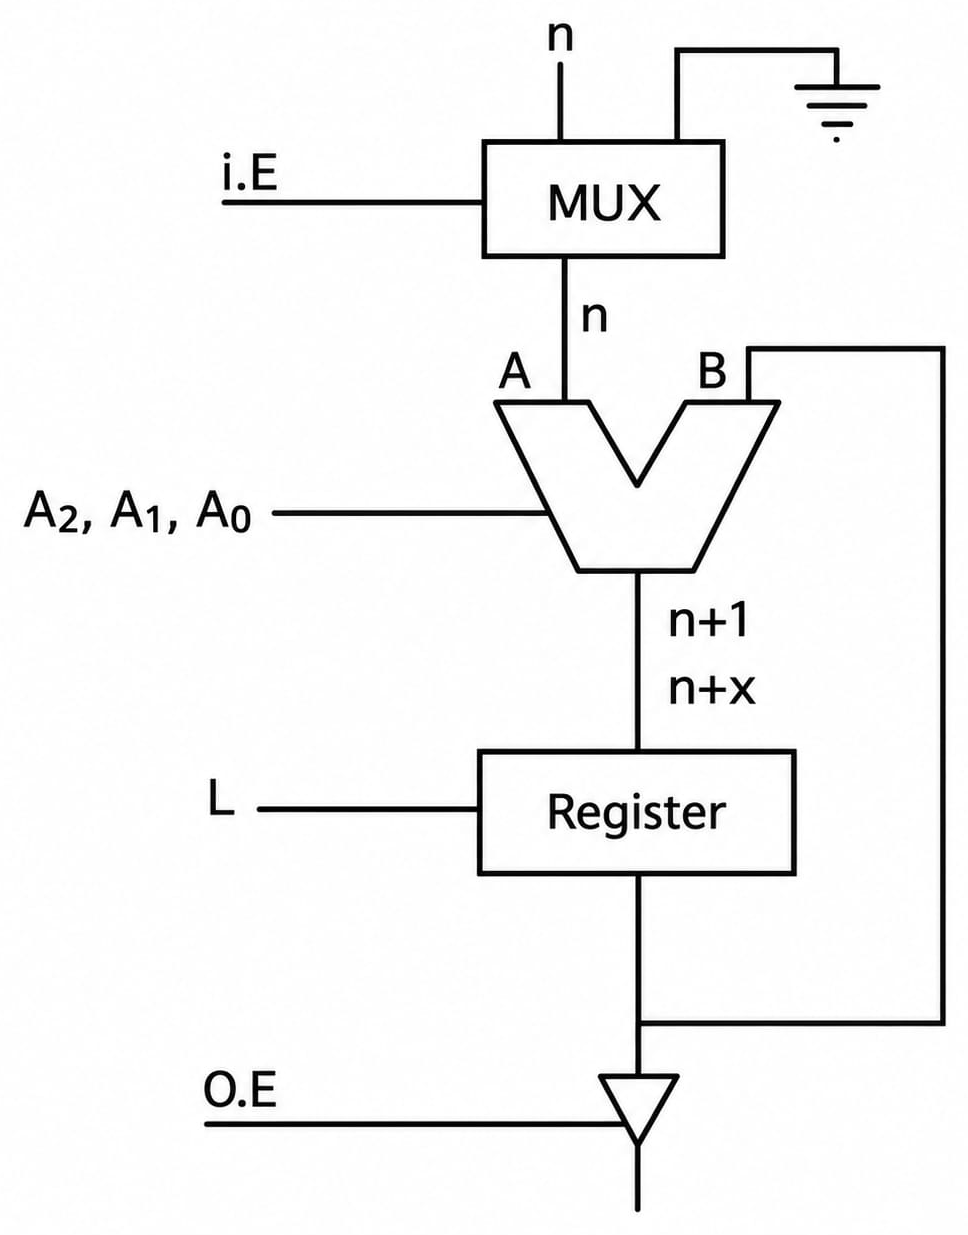
\includegraphics[width=0.70\textwidth,height=0.57\textheight,keepaspectratio]{figuras/arquitectura_datapath.png}
  \caption{Diagrama del Datapath 1 proporcionado para la practica: MUX de entrada, ALU, registro con realimentacion hacia B y buffer de salida controlado por O.E.}
  \label{fig:arquitectura}
\end{figure}

Las cuatro señales que intervienen son distintas y conviene no
confundirlas: $F_{ALU}$ es el resultado \emph{combinacional} de la ALU;
$D$ es la entrada del registro (en este diseño, el mismo cable que
$F_{ALU}$); $Q$ es el valor \emph{secuencial} almacenado, que cambia
únicamente en el flanco de reloj; y \texttt{salida} es el valor de $Q$
visible cuando \texttt{O.E}~$=1$. En forma compacta:

\begin{align*}
  A          &= \texttt{M} \mathbin{?} \texttt{dato\_ext} : 0,
    & \texttt{salida} &= \texttt{O.E} \mathbin{?} Q : \texttt{Z}, \\
  B          &= Q, &
  F_{ALU}    &= \mathrm{ALU}(A, B, C), \\
  D          &= F_{ALU}, &
  Q^{+}      &= \begin{cases}
      0   & \text{si \texttt{rst} $=1$},\\
      D   & \text{si \texttt{rst} $=0$ y \texttt{L} $=1$},\\
      Q   & \text{en otro caso},
    \end{cases}
\end{align*}

\noindent siendo $Q^{+}$ el valor que adopta el registro en cada flanco de
subida de \texttt{clk} (el reinicio tiene prioridad sobre la carga). De
esta ecuación se sigue una consecuencia temporal importante, verificada en
simulación (§\ref{sec:resultados}): con \texttt{L}~$=0$ el registro
conserva su valor y \texttt{salida} muestra el valor \emph{anterior},
aunque $F_{ALU}$ cambie por efecto de $A$, $B$ o $C$. La salida externa
sale del registro, no de la ALU.

El reinicio síncrono no aparece en la fotografía, pero es necesaria: sin
ella, $B$ no puede garantizarse en cero y la única vía de cargar
\texttt{dato\_ext} en el registro sería sumar con $B=0$ (§\ref{sec:alu-op}).
Se optó por \texttt{rst} síncrono con prioridad sobre \texttt{L}, patrón ya
usado en los registros del resto del proyecto.

\subsection{Módulos VHDL}
\label{sec:modulos}

Los modelos siguen las convenciones del proyecto: VHDL-2008
conservador~\cite{ieee1076_2008}, un fichero por entidad, paquetes
\texttt{ieee.std\_\-logic\_\-1164} y \texttt{ieee.numeric\_\-std}, y
combinación
de los estilos de descripción: \emph{dataflow} para el MUX y la ALU,
\emph{comportamental} para el registro y el buffer, y \emph{estructural}
para la integración~\cite{navabi1998vhdl}. Todos los módulos nuevos
declaran \texttt{generic ANCHO : natural := 8}, de modo que el ancho de los
buses es parametrizable y los mismos bancos de prueba pueden comprobar
anchos distintos~\cite{harris2015ddca}.

\begin{itemize}
  \item \texttt{mux\_entrada}: entradas \texttt{dato\_ext} y constante
    cero, selección \texttt{sel} (el campo \texttt{M} de la palabra de
    control, con polaridad \texttt{'1'}~$=$ dato externo, decisión de
    diseño) y salida \texttt{y}, el operando $A$.
  \item \texttt{alu}: entradas \texttt{a}, \texttt{b} y código
    \texttt{c} de 3~bits; salida \texttt{f}. Un proceso con
    \texttt{case} implementa las tres operaciones de la
    §\ref{sec:alu-op} y devuelve cero para los códigos reservados.
  \item \texttt{registro}: entradas \texttt{clk}, \texttt{rst}, \texttt{l}
    y dato \texttt{d}; salida \texttt{q}. El proceso de carga con
    prioridad de reinicio es el siguiente (extracto de
    \texttt{registro.vhd}, código completo en el Apéndice):

\begin{lstlisting}[caption={\texttt{registro.vhd} --- proceso de carga con
  prioridad de reinicio}, label=lst:registro, numbers=left]
process (clk)
begin
    if rising_edge(clk) then
        if rst = '1' then
            contenido <= (others => '0');
        elsif l = '1' then
            contenido <= d;
        end if;
    end if;
end process;
\end{lstlisting}

  \item \texttt{buffer\_salida}: entradas \texttt{d\_in} y \texttt{oe};
    salida \texttt{y} con asignación condicional:
    \texttt{y <= d\_in when oe = '1' else (others => 'Z')}.
  \item \texttt{datapath}: integración \emph{estructural} que instancia
    los cuatro módulos por componentes ---de modo que el análisis del
    conjunto no depende del orden de los ficheros---, desempaqueta la
    palabra de control (\texttt{cw(5)}=\texttt{oe}, \texttt{cw(4)}=\texttt{l},
    \texttt{cw(3)}=\texttt{m}, \texttt{cw(2~downto~0)}=\texttt{c}),
    realimenta \texttt{q} al operando \texttt{b} y declara además dos
    salidas de observación, \texttt{f\_alu} y \texttt{q\_reg}, que
    permiten inspeccionar el resultado combinacional y el valor
    almacenado en los bancos de prueba y en las capturas de ondas sin
    formar parte de la salida externa.
\end{itemize}

\subsection{Palabra de control y operaciones de la ALU}
\label{sec:alu-op}

La señal \texttt{cw} tiene 6~bits y su formato, de más significativo a
menos, es \texttt{[O.E, L, M, C2, C1, C0]}
(Tabla~\ref{tab:palabra-control}). Los
campos \texttt{O.E}, \texttt{L} y el triplete \texttt{c[0:2]} están
tomados del material del curso; la polaridad de \texttt{M} y la
correspondencia bit a bit de los campos con \texttt{cw} son decisiones de
diseño del equipo.

\begin{table}[t]
  \centering
  \caption{Formato de la palabra de control \texttt{cw} (6~bits, de MSB a
  LSB).}
  \label{tab:palabra-control}
  \footnotesize
  \begin{tabular}{clll}
    \hline
    Bits & Campo & Acción & Origen \\
    \hline
    \texttt{cw[5]} & \texttt{O.E} & habilita la salida (desde $Q$) &
      foto (\texttt{O.E.}) \\
    \texttt{cw[4]} & \texttt{L}   & carga del registro (flanco de
      \texttt{clk}) & foto (nombre provis.) \\
    \texttt{cw[3]} & \texttt{M}   & MUX: \texttt{1}=\texttt{dato\_ext},
      \texttt{0}=cero & decisión \\
    \texttt{cw[2:0]} & \texttt{C2 C1 C0} & operación de la ALU &
      foto (\texttt{c[0:2]}) \\
    \hline
  \end{tabular}
\end{table}

La Tabla~\ref{tab:alu} resume las operaciones de la ALU. Las
\emph{expresiones} ($n+x$, $2n+x$, $n+1$) provienen del material del
curso; la \emph{codificación binaria} de la columna $C$ es una propuesta
explícita y provisional del equipo, acordada para poder implementar y
verificar el diseño: la codificación original del profesor no se pudo leer
en la fotografía. Los códigos \texttt{011}--\texttt{111} quedan
reservados, y se les asigna salida cero como valor por defecto inocuo
hasta contar con evidencia de su significado real.

\begin{table}[t]
  \centering
  \caption{Operaciones de la ALU: expresiones del material del curso y
  codificación binaria propuesta (provisional) por el equipo.}
  \label{tab:alu}
  \footnotesize
  \begin{tabular}{ccccl}
    \hline
    $C$ ($c_2c_1c_0$) & Nombre & Ecuación & Usa $A$ &
      Con $A=x$, $B=n$ \\
    \hline
    \texttt{000} & suma           & $F = A + B$          & sí & $n + x$ \\
    \texttt{001} & doble y suma   & $F = (B \ll 1) + A$  & sí & $2n + x$ \\
    \texttt{010} & incremento     & $F = B + 1$          & no & $n + 1$ \\
    \texttt{011}--\texttt{111} & reservado & $F = 0$ (propuesta) & --- & --- \\
    \hline
  \end{tabular}
\end{table}

La notación $n$ y $x$ del material de clases se corresponde con los
operandos del circuito: $n$ es el contenido actual del registro, es decir,
el operando $B$; $x$ es el valor externo presente en \texttt{dato\_ext}
cuando \texttt{M}~$=1$, es decir, el operando $A$ tras el MUX. Con esa
compatibilidad, las operaciones pedidas se obtienen así: $n+x$ con
\texttt{000} y \texttt{M}~$=1$; $2n+x$ con \texttt{001} y
\texttt{M}~$=1$, usando el desplazamiento lógico a la izquierda de un bit
de $B$ \emph{dentro} de la ALU; $n+1$ con \texttt{010}, operación que
ignora $A$ y por eso hace irrelevante \texttt{M}; y la carga directa de
$x$ en el registro se consigue con un \texttt{rst} previo ($B=0$) y
\texttt{000} con \texttt{M}~$=1$, de modo que $F=x+0=x$. Como limitación
documentada, con solo estas tres operaciones no es posible cargar $A$ en
un registro cuyo $B$ sea distinto de cero: por eso el reinicio es
necesario.

\subsection{Decisiones de diseño y limitaciones}
\label{sec:decisiones}

\begin{itemize}
  \item \textbf{Ancho parametrizable}: la fotografía no permite leer el
    ancho de los buses; se adopta \texttt{ANCHO := 8} como valor por
    defecto y todos los bancos de prueba trabajan también con anchos
    distintos (por ejemplo, 4~bits) para demostrar la parametrización.
  \item \textbf{Sin banderas}: no se modelan acarreo ni indicador de
    cero. Toda la aritmética es módulo $2^{\texttt{ANCHO}}$ y los
    desbordamientos son silenciosos: con 8~bits, doblar sin pérdida
    exige $n \le 127$, y $2n+x$ sin envoltura exige $2n+x \le 255$.
    Estos límites se caracterizan empíricamente en la
    Sección~\ref{sec:resultados}.
  \item \textbf{Sin FSM, sin shifter externo}: únicamente los módulos del
    esquema del curso más \texttt{clk} y \texttt{rst}.
  \item \textbf{Solo simulación}: todas las fuentes se verificaron
    \emph{exclusivamente} por simulación con GHDL (backend \texttt{mcode}).
    GHDL dispone de un flujó experimental de síntesis
    (\texttt{ghdl {-}{-}synth})~\cite{ghdl-docs}; en este proyecto no se
    \emph{utilizó} ese flujo ni se evaluaron la síntesis ni la
    implementación física, por lo que no se afirma sintetizabilidad.
\end{itemize}

% ============================================================
% 3. PROPUESTA EXPERIMENTAL  (1 hoja)
% ============================================================
\section{Propuesta Experimental}
\label{sec:propuesta}

La metodología sigue un flujo descendente: de la especificación de la
§\ref{sec:diseno} se pasó a los modelos VHDL-2008, después a la
integración estructural y, en paralelo, a los bancos de prueba; la
verificación se hizo por simulación y el análisis de resultados por
inspección de ondas. Los modelos combinan los estilos \emph{dataflow},
\emph{comportamental} y \emph{estructural}~\cite{navabi1998vhdl} y sus
procesos siguen las sentencias secuenciales del lenguaje~\cite{ashenden2008vhdl},
con un estilo de diseño y de entidades consistente con el de los textos de
referencia del curso~\cite{harris2015ddca,ieee1076_2008}.

Las herramientas de simulación son GHDL~\cite{ghdl-docs}, invocado con el
estándar \texttt{--std=08} y volcado de ondas a formato VCD, y
GTKWave~\cite{gtkwave-docs} para la inspección de las ondas y la
exportación de capturas mediante scripts Tcl. La ejecución se apoya en los
scripts oficiales del repositorio: \texttt{vhdl-analizar} analiza las
fuentes, \texttt{vhdl-sim} analiza, elabora y ejecuta cada banco de
prueba, y \texttt{latexbuild} compila este informe en formato Springer
(llncs).

Se definieron cinco bancos de prueba autochequeados, uno por módulo y uno
de integración:

\begin{itemize}
  \item \texttt{tb\_mux\_entrada}: comprueba todas las selecciones del MUX
    con el genérico \texttt{ANCHO} igual a 8 y a 4~bits.
  \item \texttt{tb\_registro}: verifica el reinicio, la carga con
    \texttt{L} y la retención cuando \texttt{L}~$=0$.
  \item \texttt{tb\_buffer\_salida}: comprueba que con \texttt{oe}~$=1$
    propaga el dato y con \texttt{oe}~$=0$ entrega alta impedancia.
  \item \texttt{tb\_alu}: 27~comprobaciones sobre las tres operaciones
    (incluidos operandos nulos y máximos), los desbordamientos
    ($200+100$ sobre 8~bits, $200 \ll 1$ con pérdida del bit más
    significativo, $255+1$ envolviendo a cero), los códigos reservados y
    un segundo ejemplo con \texttt{ANCHO} igual a 4~bits.
  \item \texttt{tb\_datapath}: aplica las cinco palabras de control
    verificadas, reproduce el ejemplo completo de tres ciclos
    ($x=5$ con reinicio inicial) y ejecuta la prueba discriminante
    \texttt{L}~$=0$: con \texttt{CW = 100010} la ALU calcula $n+1$,
    pero la salida externa debe seguir siendo $n$.
\end{itemize}

Cada banco de prueba termina siempre con un mensaje de éxito
(\texttt{tb\_...: OK}) y falla con \texttt{assert ... severity failure}
ante cualquier desviación respecto al valor esperado. El pulso de reloj se
genera dentro del proceso estimulador ---patrón de todos los bancos de
prueba del proyecto, ya que \texttt{vhdl-sim} no impone un límite
de tiempo---, de modo que toda simulación termina de forma
determinista. Además, la integración continua del repositorio ejecuta la
batería completa de \texttt{tb\_*.vhd} en cada cambio.

El procedimiento de evaluación, repetido para cada experimento, fue:
(1)~analizar la unidad con el script \texttt{vhdl-analizar};
(2)~ejecutar el banco de prueba con \texttt{vhdl-sim} y comprobar en
consola que termina con \texttt{OK} y sin errores de GHDL;
(3)~volcar el VCD resultante;
(4)~capturar las ondas relevantes a PNG con GTKWave; y (5)~contrastar los
valores esperados y observados de las señales. Criterio de éxito: los
cinco bancos terminan con \texttt{OK} y ninguna aserción se dispara. Los
casos en que el resultado aritmético difiere del valor matemático exacto
por envoltura módulo $2^{\texttt{ANCHO}}$ no se consideran fallos, sino
comportamiento documentado en la Sección~\ref{sec:decisiones} y analizado
en la Sección~\ref{sec:resultados}.

% ============================================================
% 4. SIMULACIONES DE VHDL  (capturas de los módulos más importantes)
% ============================================================
\section{Simulaciones de VHDL}
\label{sec:simulaciones}

Las capturas que siguen se obtuvieron ejecutando los bancos de prueba con
\texttt{scripts/vhdl-sim datapath-1 <tb>}, que vuelca las ondas en
\texttt{vhdl/datapath-1/salidas/<tb>.vcd}, y abriéndolas después en GTKWave
mediante un script Tcl que fija el rango de tiempos visible, el orden de las
señales y exporta el PNG a \texttt{figuras/}. Para que la fuente sea
legible, cada figura recorta una ventana corta de la traza; los valores que
se leen en las ondas coinciden con las aserciones del banco de prueba
correspondiente.

La Fig.~\ref{fig:ondas-datapath} muestra el tramo principal de la
simulación del datapath completo (5--95~ns), con las señales \texttt{clk},
\texttt{rst}, \texttt{dato\_ext}, \texttt{cw}, \texttt{f\_alu},
\texttt{q\_reg} y \texttt{salida}. En el primer ciclo (tras el reinicio de
la traza, a $t\approx 10$~ns) la palabra de control \texttt{111000} carga
$n=5$: \texttt{f\_alu} pasa a \texttt{0x05} de forma combinacional y, en el
flanco, \texttt{q\_reg} y \texttt{salida} se actualizan a \texttt{0x05}.
En el segundo ciclo, \texttt{111001} ($2n+x$) lleva \texttt{f\_alu} a
\texttt{0x0F} y el registro a \texttt{0x0F}. El tramo central
($\approx$50--65~ns) es la prueba discriminante: con \texttt{CW=100010}
($L=0$, $n+1$) la ALU calcula \texttt{f\_alu=0x10}, pero \texttt{q\_reg} y
\texttt{salida} permanecen en \texttt{0x0F} incluso después del flanco,
porque el registro no carga.

\begin{figure}[t]
  \centering
  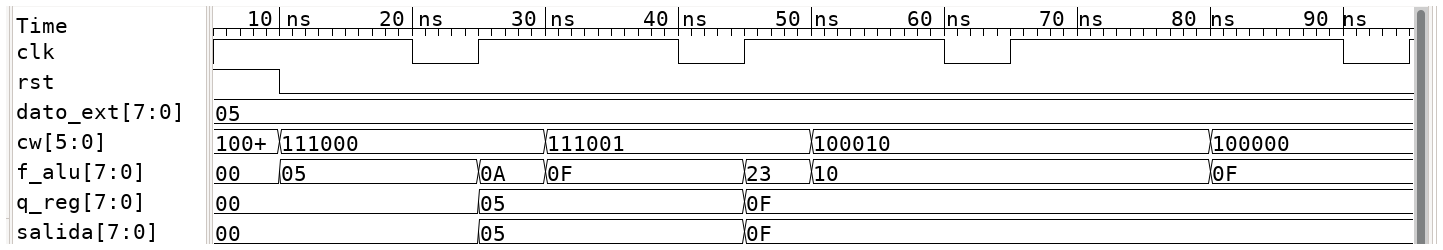
\includegraphics[width=\textwidth]{figuras/tb-datapath-ondas.png}
  \caption{Simulación del datapath completo (\texttt{tb\_datapath}),
  ventana de 5--95~ns. Se aprecia la actualización de \texttt{q\_reg} y
  \texttt{salida} solo en los flancos con \texttt{L}=1 y, en el tramo
  central, que con \texttt{L}=0 la salida no sigue a \texttt{f\_alu}: la
  salida proviene del registro.}
  \label{fig:ondas-datapath}
\end{figure}

La salida del buffer en tramo de alta impedancia queda en la
Fig.~\ref{fig:ondas-datapath-salida}, que recorta la ventana final de la
misma simulación (105--170~ns). Al cargar \texttt{dato\_ext=0x3C} con
\texttt{CW=011000} ($\mathtt{O.E}=0$), \texttt{salida} está en estado $Z$;
la palabra de control \texttt{100000} habilita el buffer y muestra el
valor guardado; y, por último, \texttt{n+1} con \texttt{CW=110010} lleva el
registro a \texttt{0x3D}, visible bajo \texttt{q\_reg}, \texttt{f\_alu} y
\texttt{salida}. Esta ventana es la contraprueba del capítulo de
arquitectura: la carga con \texttt{L}=1 y la baja a alta impedancia con
$\mathtt{O.E}=0$ confirman que el registro y el buffer separan el
almacenamiento del \emph{drive}.

\begin{figure}[t]
  \centering
  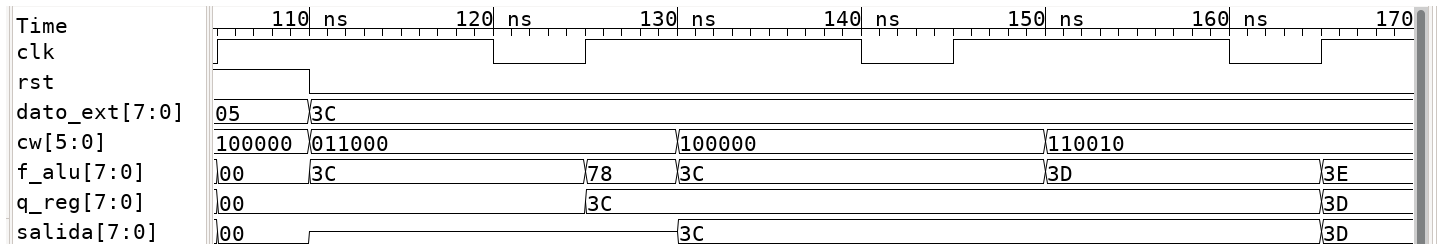
\includegraphics[width=\textwidth]{figuras/tb-datapath-salida.png}
  \caption{Simulación del datapath completo (\texttt{tb\_datapath}),
  ventana de 105--170~ns. Con \texttt{CW=011000} la salida está en alta
  impedancia ($Z$); \texttt{100000} restaura el buffer con el valor
  guardado y \texttt{110010} ($n+1$) lo actualiza a \texttt{0x3D}.}
  \label{fig:ondas-datapath-salida}
\end{figure}

La Fig.~\ref{fig:ondas-alu} presenta la simulación de la ALU en su
instancia de 8~bits (95--170~ns), con las señales \texttt{a8}, \texttt{b8},
\texttt{c} y \texttt{f8}. Se ve el barrido de las tres operaciones ---suma
(\texttt{c=000}), doble y suma (\texttt{c=001}) e incremento
(\texttt{c=010})--- y los tres desbordamientos documentados en la
Sección~\ref{sec:decisiones}: \texttt{100+200=0x2C}, \texttt{200}$\ll$%
1\texttt{=0x90} y \texttt{255+1=0x00}, todos por envoltura módulo $2^8$.
 Los cinco códigos reservados del barrido y la instancia de 4~bits
devuelven \texttt{0}; su formulario está tabulado en la
Tabla~\ref{tab:res-alu}.

\begin{figure}[t]
  \centering
  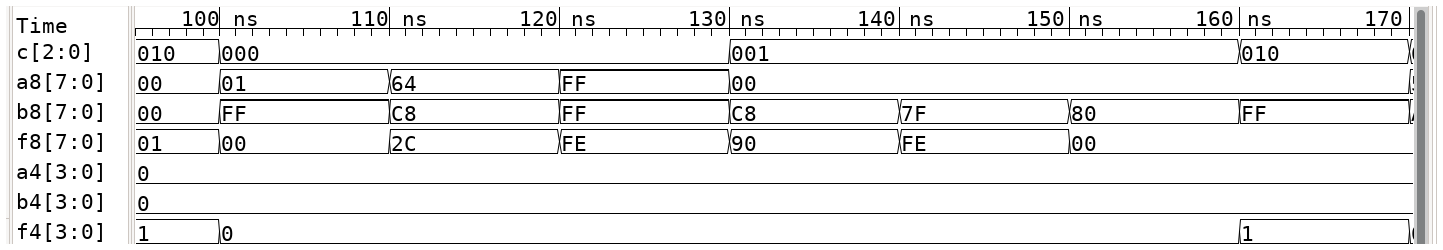
\includegraphics[width=\textwidth]{figuras/tb-alu-ondas.png}
  \caption{Simulación de la ALU (\texttt{tb\_alu}) en 8~bits
  (\texttt{a8}, \texttt{b8}, \texttt{f8}), ventana de 95--170~ns. El código
  \texttt{c} recorre las tres operaciones y los tres desbordamientos, que
  envuelven módulo $2^8$.}
  \label{fig:ondas-alu}
\end{figure}

Por último, la Fig.~\ref{fig:alu-ancho4} recoge la ventana de la instancia
de 4~bits de la misma simulación (215--250~ns), en la que se verifica que
el modelo es genérico respecto al parámetro \texttt{ANCHO}: \texttt{3+1=4},
\texttt{9}$\ll$1\texttt{=2} ($18 \bmod 16$) y \texttt{15+1=0}. Las demás
capturas ---\texttt{tb\_mux\_entrada} y \texttt{tb\_buffer\_salida}---
confirman el comportamiento combinacional de los bloques restantes y no
se muestran por límite de espacio.

\begin{figure}[t]
  \centering
  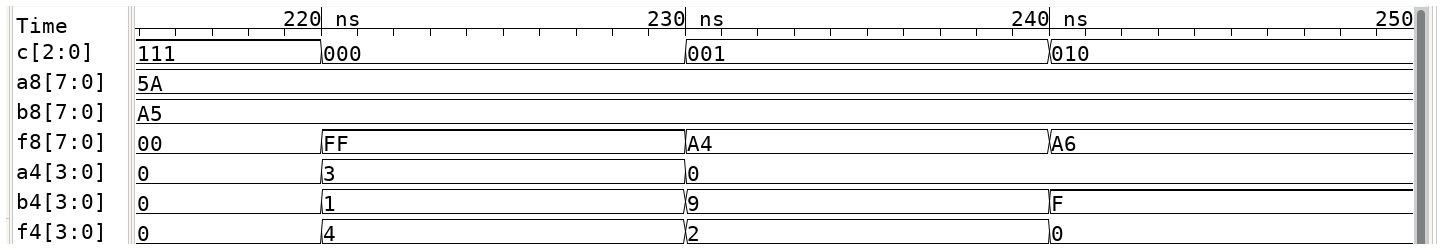
\includegraphics[width=\textwidth]{figuras/tb-alu-ancho4.png}
  \caption{Simulación de la ALU (\texttt{tb\_alu}) en 4~bits
  (\texttt{a4}, \texttt{b4}, \texttt{f4}), ventana de 215--250~ns. Las
  mismas tres operaciones en \texttt{ANCHO}=4: \texttt{3+1=4},
  \texttt{9$\ll$1=2} y \texttt{15+1=0} muestran la envoltura módulo $2^4$.}
  \label{fig:alu-ancho4}
\end{figure}

% ============================================================
% 5. RESULTADOS  (3–5 cuartillas)
% ============================================================
\section{Resultados}
\label{sec:resultados}

\subsection{Ejecución de los bancos de prueba}

Los cinco bancos de prueba se ejecutaron con el script
\texttt{vhdl-sim} del repositorio y todos terminaron con el
mensaje de éxito, sin que se disparase ninguna aserción
(Tabla~\ref{tab:tbs}). El instante final es el del \texttt{report ... OK},
que depende del número de estímulos de cada banco y no de un tiempo de
simulación impuesto por la herramienta, ya que el reloj se genera dentro
del propio proceso estimulador.

\begin{table}[t]
  \centering
  \caption{Resultado de la ejecución de los cinco bancos de prueba
  (\texttt{scripts/vhdl-sim datapath-1 <tb>}).}
  \label{tab:tbs}
  \footnotesize
  \begin{tabular}{llcl}
    \hline
    Banco de prueba & Módulo bajo prueba & Fin & Resultado \\
    \hline
    \texttt{tb\_mux\_entrada}  & \texttt{mux\_entrada}  & 60~ns  & OK \\
    \texttt{tb\_registro}      & \texttt{registro}      & 50~ns  & OK \\
    \texttt{tb\_buffer\_salida}& \texttt{buffer\_salida}& 40~ns  & OK \\
    \texttt{tb\_alu}           & \texttt{alu}           & 250~ns & OK (27 aserciones) \\
    \texttt{tb\_datapath}      & \texttt{datapath}      & 170~ns & OK \\
    \hline
  \end{tabular}
\end{table}

También se verificó el análisis de todas las fuentes y bancos de prueba
con \texttt{scripts/vhdl-analizar datapath-1} (cinco fuentes y cinco
bancos), sin mensajes de error de GHDL~4.1.0 con el estándar
\texttt{--std=08}. La integración continua del repositorio reproduce esta
misma batería.

\subsection{Operaciones de la ALU}

La Tabla~\ref{tab:res-alu} recoge, para una muestra representativa de los
27~casos comprobados, el valor de los operandos, el código y el resultado
observado, con el resultado matemático de referencia. Los tres
desbordamientos documentados en la Sección~\ref{sec:decisiones} se
manifiestan como desbordamiento modular (envoltura) de módulo $2^8$: $200+100$ da \texttt{0x2C} (=~44),
porque $300 \bmod 256 = 44$; doblar $200$ da \texttt{0x90} (=~144),
porque $400 \bmod 256 = 144$; y $255+1$ da \texttt{0x00}. Ninguno de estos
casos es un fallo del modelo, sino la consecuencia de trabajar sin banderas
de acarreo ni de desbordamiento.

La instancia con \texttt{ANCHO}=4 (filas inferiores de la
Tabla~\ref{tab:res-alu}) confirma que el \emph{generic} parametriza la
ruta aritmética completa y no solo los anchos de los puertos. Las tres
operaciones se repiten con operandos de 4~bits y los límites se desplazan
de $2^8-1=255$ a $2^4-1=15$: $3+1=4$ cabe sin envolver, $2\cdot9=18 \equiv 2 \pmod{16}$ y $15+1=0$. El
resultado observado coincide en los tres casos con la referencia
matemática, lo que valida la parametrización del diseño sin cambios de
descripción (es la misma entidad \texttt{alu} instanciada con otro valor
del \emph{generic}).

\begin{table}[t]
  \centering
  \caption{Resultados de la ALU observados en \texttt{tb\_alu}
  (extracto de los 27~casos; 8~bits salvo indicación).}
  \label{tab:res-alu}
  \footnotesize
  \begin{tabular}{cccccl}
    \hline
    $C$ & $A$ & $B=n$ & $F$ observado & Referencia & Observación \\
    \hline
    \texttt{000} & \texttt{0A} & \texttt{05} & \texttt{0F} & $5+10=15$ & $n+x$ \\
    \texttt{000} & \texttt{3C} & \texttt{00} & \texttt{3C} & $x+0$ & carga de $x$ \\
    \texttt{001} & \texttt{0A} & \texttt{05} & \texttt{14} & $2\cdot5+10=20$ & $2n+x$ \\
    \texttt{001} & \texttt{00} & \texttt{7F} & \texttt{FE} & $2\cdot127=254$ & límite exacto \\
    \texttt{010} & \texttt{A5} & \texttt{05} & \texttt{06} & $5+1=6$ & ignora $A$ \\
    \texttt{000} & \texttt{64} & \texttt{C8} & \texttt{2C} & $300 \bmod 256$ & \textbf{envoltura} ($=44$) \\
    \texttt{001} & \texttt{00} & \texttt{C8} & \texttt{90} & $400 \bmod 256$ & \textbf{envoltura} ($=144$) \\
    \texttt{010} & \texttt{00} & \texttt{FF} & \texttt{00} & $256 \bmod 256$ & \textbf{envoltura} \\
    \texttt{011}--\texttt{111} & \texttt{5A} & \texttt{A5} & \texttt{00} & reservado & valor por defecto \\
    \hline
    \multicolumn{6}{l}{\emph{Instancia con \texttt{ANCHO}=4:}}\\
    \texttt{000} & \texttt{0011} & \texttt{0001} & \texttt{0100} & $3+1=4$ & $n+x$ \\
    \texttt{001} & \texttt{0000} & \texttt{1001} & \texttt{0010} & $18 \bmod 16$ & $2n+x$ ($=2$) \\
    \texttt{010} & \texttt{0000} & \texttt{1111} & \texttt{0000} & $16 \bmod 16$ & \textbf{envoltura} \\
    \hline
  \end{tabular}
\end{table}

\subsection{Palabras de control en el datapath}

La Tabla~\ref{tab:res-cw} contrasta, para cada palabra de control
empleada, el resultado esperado con el observado en \texttt{tb\_datapath}.
Las filas de los ciclos 1 y 2 corresponden al ejemplo de tres ciclos de la
Sección~\ref{sec:alu-op}; la prueba discriminante (\texttt{CW=100010})
confirma que con \texttt{L}=0 la salida externa conserva el valor del
registro y no adopta el nuevo resultado de la ALU. La carga con
\texttt{CW=011000} muestra además la alta impedancia cuando
$\mathtt{O.E}=0$.

\begin{table}[t]
  \centering
  \caption{Resultados del datapath observados en \texttt{tb\_datapath}
  (valores en hexadecimal).}
  \label{tab:res-cw}
  \footnotesize
  \begin{tabular}{ccccccc}
    \hline
    \texttt{CW} & \multicolumn{2}{c}{$F_{ALU}$} &
      \multicolumn{2}{c}{$Q$} & \texttt{salida} & Observación \\
    & \emph{esp.} & \emph{obs.} & \emph{esp.} & \emph{obs.}
      & & \\
    \hline
    \texttt{111000} & \texttt{05} & \texttt{05} & \texttt{05} &
      \texttt{05} & \texttt{05} & $n+x$ guardado \\
    \texttt{111001} & \texttt{0F} & \texttt{0F} & \texttt{0F} &
      \texttt{0F} & \texttt{0F} & $2n+x$ guardado \\
    \texttt{100010} & \texttt{10} & \texttt{10} & \texttt{0F} &
      \texttt{0F} & \texttt{0F} & $L=0$: salida $=$ registro \\
    \texttt{100000} & \texttt{0F} & \texttt{0F} & \texttt{0F} &
      \texttt{0F} & \texttt{0F} & conservar y mostrar \\
    \texttt{011000} & \texttt{3C} & \texttt{3C} & \texttt{3C} &
      \texttt{3C} & \texttt{Z} & carga con $\mathtt{O.E}=0$ \\
    \texttt{110010} & \texttt{3D} & \texttt{3D} & \texttt{3D} &
      \texttt{3D} & \texttt{3D} & $n+1$ guardado \\
    \hline
  \end{tabular}
\end{table}

En todos los casos el valor observado de $F_{ALU}$ y el del registro tras
el flanco coinciden con el esperado. El interés de la fila
\texttt{100010} es que el registro y la ALU divergen deliberadamente:
$F_{ALU}=\texttt{0x10}$, pero $Q=\texttt{salida}=\texttt{0x0F}$, lo que
valida la corrección de diseño de la §\ref{sec:arquitectura} (la salida
sale del registro).

\subsection{Comportamiento temporal}

Del análisis de las ondas (Fig.~\ref{fig:ondas-datapath}) se desprenden
dos observaciones. Primero, la latencia del resultado es de un flanco:
cuando \texttt{L}=1, el valor nuevo de $F_{ALU}$ está disponible de forma
combinacional en el mismo ciclo, pero solo se hace visible en \texttt{salida}
tras el flanco de subida, porque atraviesa el registro. Segundo, la salida
combinacional de la ALU ($F_{ALU}$) sí puede cambiar en cualquier momento
del ciclo al variar $A$, $B$ o $C$; por eso se expone como salida de
observación \texttt{f\_alu}, separada de la salida externa. El diseño
resulta así coherente con la separación entre la parte combinacional y la
secuencial, y con el modelo de la §\ref{sec:arquitectura}.

Las ventanas dedicadas a la ALU refuerzan la lectura combinacional.
En la Fig.~\ref{fig:ondas-alu}, \texttt{f8} responde a cada cambio de
\texttt{c8} o de los operandos en el instante exacto del cambio, sin
esperar flanco de reloj alguno: la suma $100+200$ produce \texttt{0x2C},
doblar $200$ produce \texttt{0x90} y el caso límite
$255+1$ produce \texttt{0x00} en su correspondiente ventana. Por su
parte, la Fig.~\ref{fig:alu-ancho4} recoge el mismo banco con
\texttt{ANCHO}=4 en el tramo final: \texttt{c4} recorre el código
reservado (\texttt{111}, con \texttt{f4}=0) y después las tres
operaciones de la Tabla~\ref{tab:res-alu} ($3+1=4$; $2\cdot9 \equiv 2 \pmod{16}$; $15+1=0$), mientras la instancia de 8 bits sigue
estimulada en paralelo con sus propios operandos (\texttt{f8} responde a
sus estímulos en las mismas ventanas). Ambas ventanas ilustran, además,
un rasgo del entorno de simulación: la regla temporal en nanosegundos y
el escalado automático (\emph{zoom}) dependen de la herramienta, no del
modelo VHDL de \texttt{vhdl/datapath-1}.

En cuanto a coste, y sin entrar en síntesis (el flujo es solo simulación),
el datapath resuelve cada micro-operación en un único ciclo de reloj,
salvo la secuencia de inicialización que requiere un \texttt{rst} previo
para poder cargar \texttt{dato\_ext} con $B=0$. No hay por tanto
operaciones que abarquen varios ciclos ni \emph{overhead} de una máquina de
estados,
a cambio de que la secuencia la deba aportar el entorno externo; desde la
perspectiva de las métricas de rendimiento clásicas, el tiempo de
ejecución de una secuencia es proporcional al número de palabras de
control aplicadas~\cite{stallings2015coa,hennessy2017qa}.

\subsection{Discusión}

Los resultados confirman el funcionamiento previsto y, al mismo tiempo,
delimitan las limitaciones que ya se anticiparon en el diseño. La más
importante es la aritmética silenciosa: al no haber banderas, el modelo no
distingue un resultado correcto de uno envuelto, de modo que la validez de
$2n+x$ y de $n+x$ queda condicionada a los rangos indicados en la
Sección~\ref{sec:decisiones} ($n \le 127$ para doblar sin pérdida, y
$2n+x \le 255$ en 8~bits). La segunda es la imposibilidad de cargar
$A$ sobre un registro con $B \neq 0$ usando solo las tres operaciones
pedidas; se resuelve con el reinicio, que es una decisión de diseño
adicional y no un elemento del esquema original. Por último, la
codificación binaria de la ALU es provisional: el comportamiento del
modelo es correcto \emph{bajo esa codificación}, pero si el material del
curso fija otra, habría que reajustar la tabla y repetir la verificación.
Los bancos de prueba están escritos de forma que ese cambio afectaría solo
a la tabla de la §\ref{sec:alu-op} y a los estímulos de \texttt{tb\_alu} y
\texttt{tb\_datapath}.

% ============================================================
% 6. CONCLUSIONES  (1 cuartilla)
% ============================================================
\section{Conclusiones}
\label{sec:conclusiones}

Se diseñó y verificó por simulación el Datapath 1: una ruta de datos de
8~bits parametrizable, compuesta por un MUX $2\to1$, una ALU de tres
operaciones, un registro con carga y un buffer tri-estado de salida,
integrados de forma estructural y realimentados del registro hacia la ALU.
Los cinco objetivos planteados en la introducción se cumplieron: los
módulos se describieron en VHDL-2008 con ancho parametrizable, se
integraron en una entidad estructural, se verificaron con cinco bancos de
prueba autochequeados y se analizó su comportamiento temporal a partir de
las ondas de GTKWave.

El resultado principal es una ruta de datos correcta bajo el modelo
especificado: las tres operaciones ($n+x$, $2n+x$ y $n+1$), la carga del
registro, la retención con \texttt{L}=0 y la alta impedancia con
$\mathtt{O.E}=0$ se comportan como se esperaba, incluidos los casos de
desbordamiento documentados. La decisión de diseño que separa el resultado
combinacional de la ALU ($F_{ALU}$) del valor almacenado ($Q$) quedó
validada por la prueba discriminante con \texttt{CW=100010}: con la carga
deshabilitada, la salida externa no sigue a la ALU.

Las principales limitaciones son tres y quedan documentadas: los
desbordamientos son silenciosos al no modelarse banderas; solo las tres
operaciones pedidas están implementadas, de modo que cargar el operando
externo sobre un registro no nulo exige un reinicio previo; y la
codificación binaria de la ALU y el formato exacto de la palabra de control
son una propuesta del equipo mientras no se disponga de la codificación
original. El modelo es, además, una descripción para simulación: los
códigos se verificaron \emph{únicamente} por simulación; el flujo de
síntesis experimental de GHDL (\texttt{ghdl {-}{-}synth}) no se empleó y
la sintetizabilidad y la implementación física no se han evaluado.

Como trabajo futuro inmediato cabe refactorizar tan pronto como se
disponga de la codificación real del curso (una rama por cambio, según el
flujo del repositorio), añadir banderas de acarreo y de cero preservando
la realimentación, y dotar al datapath de una unidad de control mínima
---una máquina de estados de estilo Moore o Mealy--- que genere la
secuencia de palabras de control que aquí aplica el banco de prueba. Una
unidad de control así ampliaría el funcionamiento del datapath (secuen-
ciar microoperaciones sin seguir aplicando \texttt{cw} a mano), aunque por
sí sola no bastaría para constituir un procesador completo: faltarían
elementos propios de un procesador, como una memoria de instrucciones,
un contador de programa y formateo/carga de la unidad de datos.

% ============================================================
% REFERENCIAS  (>= 15 — indicar exactamente dónde aparece el texto)
% ============================================================
% IMPORTANTE: cada referencia debe permitir ubicar exactamente dónde
% aparece el texto sugerido (capítulo/§/página, o URL + fecha de consulta).
% Anota la ubicación en un comentario % justo debajo de la entrada.
\bibliographystyle{splncs04}
\bibliography{referencias}

% ============================================================
% APÉNDICE — CÓDIGO VHDL
% ============================================================
\appendix
\section{Código VHDL}
\label{app:codigo}

Se reproduce a continuación el código completo de los módulos de la
unidad que se han verificado en este informe. Se inserta desde las copias
de presentación guardadas en \texttt{apendice/}, con el código idéntico
al VHDL funcional de \texttt{vhdl/datapath-1/src/} (misma lógica, mismos
recursos y mismos puertos) salvo los saltos de línea, ajustados a límites
sintácticos para que las instrucciones se puedan leer y copiar sin
ambigüedad, y los comentarios, reformateados al mismo ancho y redactados
en términos técnicos neutros.

\lstinputlisting[caption={\texttt{mux\_entrada.vhd} --- MUX $2\to1$ de
  entrada}, label=lst:mux]{apendice/mux_entrada.vhd}

\lstinputlisting[caption={\texttt{alu.vhd} --- ALU con las tres
  operaciones y códigos reservados a cero}, label=lst:alu]{apendice/alu.vhd}

\lstinputlisting[caption={\texttt{registro.vhd} --- registro con carga y
  reinicio síncrono}, label=lst:registro-ap]{apendice/registro.vhd}

\lstinputlisting[caption={\texttt{buffer\_salida.vhd} --- buffer
  tri-estado con habilitación}, label=lst:buffer-ap]{apendice/buffer_salida.vhd}

\lstinputlisting[caption={\texttt{datapath.vhd} --- integración
  estructural, desempaquetado de \texttt{cw} y realimentación},
  label=lst:datapath-ap]{apendice/datapath.vhd}

\end{document}
